\chapter{Pilhas e eletrólise}\label{ch:g12:cells-and-electrolysis}

Um celular mostra 1 \% numa noite de inverno e desliga. Ligado na tomada
durante a noite, de manhã ele está carregado de novo. Dentro da sua
bateria, a mesma \omterm{def:g7:chemical-reactions:reaction}{reação química} acontece num sentido durante o dia,
fornecendo energia elétrica, e é forçada no outro sentido à noite pelo
carregador. Uma \omterm{def:g11:redox:reaction}{reação de oxirredução} vira uma fonte de eletricidade
quando os seus \omterm{def:g9:inside-the-atom:nucleus}{elétrons} são obrigados a passar por um fio; e a
eletricidade, empurrada através de uma solução, pode forçar uma \omterm{def:g11:redox:reaction}{reação
de oxirredução} que nunca aconteceria sozinha.

\begin{recall}
Os \omterm{def:g11:redox:oxidant}{oxidantes} ganham \omterm{def:g9:inside-the-atom:nucleus}{elétrons}, os \omterm{def:g11:redox:oxidant}{redutores} os perdem; \omterm{def:g11:redox:couple}{semirreações},
\omterm{def:g11:redox:couple}{pares redox} e \omterm{def:g11:redox:reaction}{reações de oxirredução} (\cref{ch:g11:redox}). Um sistema
evolui até $Q = K$ (\cref{ch:g12:equilibrium}). As soluções de \omterm{def:g9:ions:ion}{íons}
conduzem (\cref{ch:g9:ions}); o \omterm{def:g10:the-mole:amount}{mol} e a \omterm{def:g10:the-mole:avogadro}{constante de Avogadro}
(\cref{ch:g10:the-mole}).
\end{recall}

\begin{omfigure}
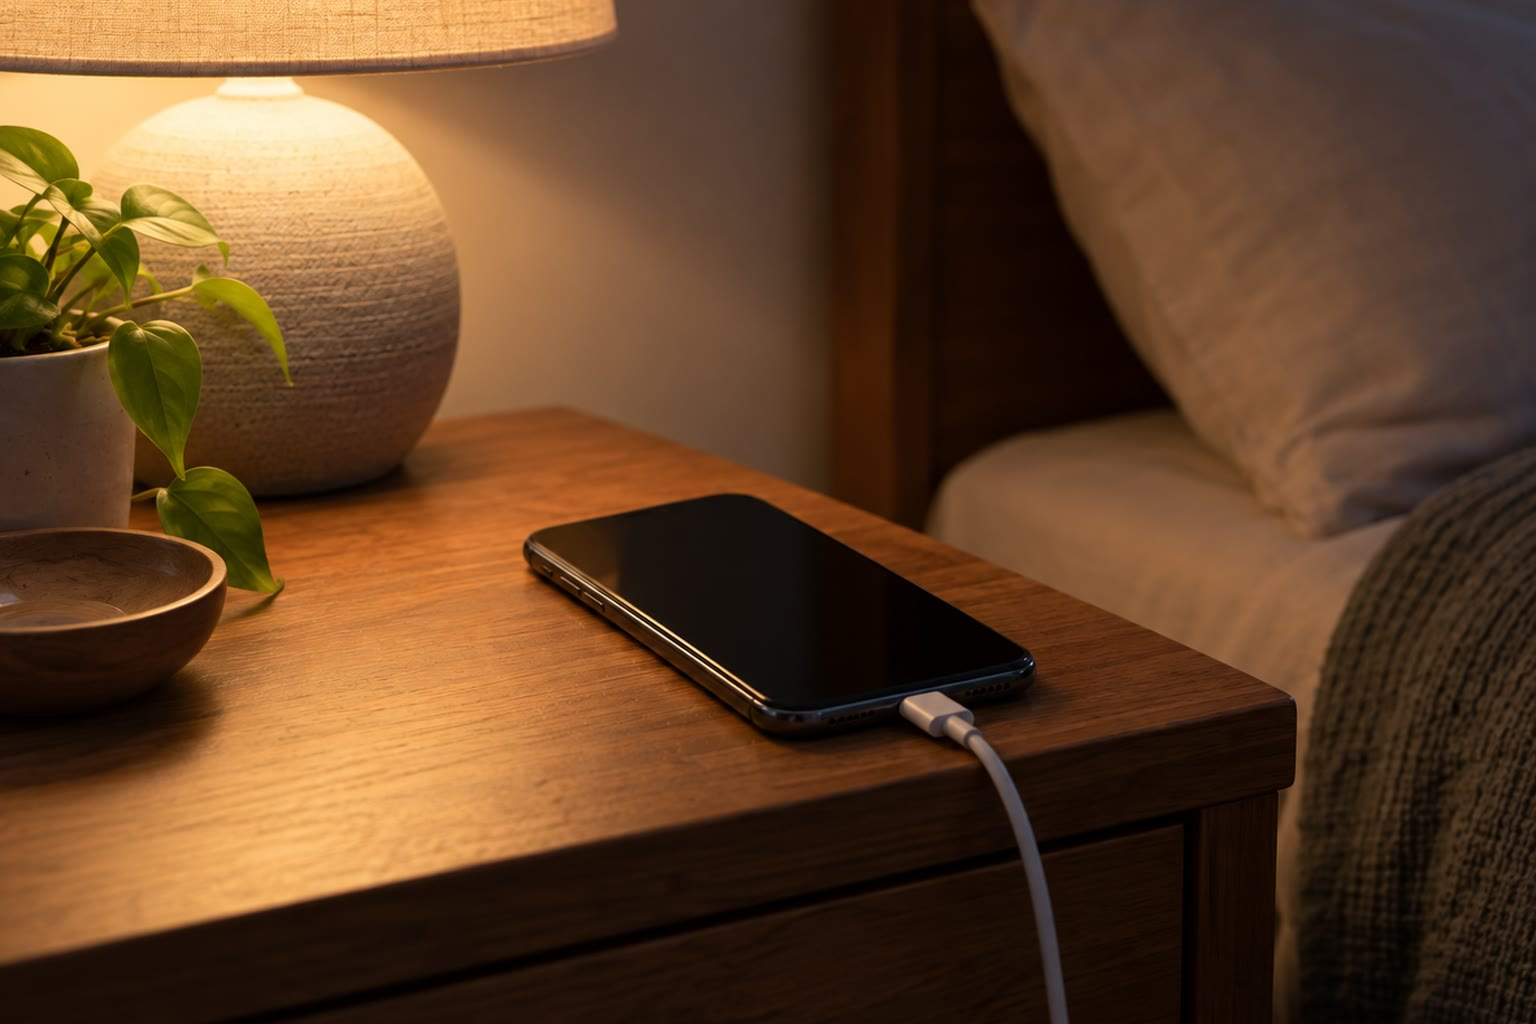
\includegraphics[width=0.45\linewidth]{images/book1/ai/g12-phone-charging.jpg}

{\small Carregar um celular: uma reação forçada no sentido inverso
durante a noite.}
\end{omfigure}

\section{Uma reação de oxirredução dividida em duas}

Quando uma lâmina de zinco é mergulhada numa solução de sulfato de
cobre, o zinco é oxidado e os \omterm{def:g9:ions:ion}{íons} cobre são reduzidos na superfície da
lâmina, \ce{Zn + Cu^{2+} -> Zn^{2+} + Cu}: os \omterm{def:g9:inside-the-atom:nucleus}{elétrons} passam
diretamente do \omterm{def:g9:periodic-table-first-look:metal}{metal} para os \omterm{def:g9:ions:ion}{íons}, e a energia se perde como um pouco de
calor. Separe as duas metades e ligue-as por um fio: os \omterm{def:g9:inside-the-atom:nucleus}{elétrons} agora
têm de passar pelo fio, e podem acender uma lâmpada no caminho.

\begin{definition}[Pilha eletroquímica, meia-pilha, ponte salina]\label{def:g12:cells-and-electrolysis:cell}
Uma \emph{pilha eletroquímica}\index{pilha eletroquimica@pilha eletroquímica} produz energia
elétrica a partir de uma \omterm{def:g11:redox:reaction}{reação de oxirredução} cuja \omterm{def:g11:redox:oxidation}{oxidação} e cuja
\omterm{def:g11:redox:oxidation}{redução} acontecem em dois compartimentos separados. Cada compartimento,
um eletrodo de \omterm{def:g9:periodic-table-first-look:metal}{metal} mergulhado numa solução dos seus \omterm{def:g9:ions:ion}{íons}, é uma
\emph{meia-pilha}\index{meia-pilha}. Uma \emph{ponte
salina}\index{ponte salina}, um tubo ou uma tira de papel embebida numa
solução de \omterm{def:g9:ions:ion}{íons}, liga as duas soluções e fecha o circuito, mantendo-as
separadas.
\end{definition}

\begin{definition}[Ânodo, cátodo]\label{def:g12:cells-and-electrolysis:anode}
O eletrodo onde acontece uma \omterm{def:g11:redox:oxidation}{oxidação} é o \emph{ânodo}\index{anodo@ânodo}; o
eletrodo onde acontece uma \omterm{def:g11:redox:oxidation}{redução} é o \emph{cátodo}\index{catodo@cátodo}.
\end{definition}

\begin{omfigure}
\begin{tikzpicture}[font=\small, scale=1.25]
  \pic[transform shape] at (0,0) {beaker={0.7}{black!6}};
  \pic[transform shape] at (4,0) {beaker={0.7}{cyan!70!blue!35}};
  \pic[transform shape] (zn) at (-0.3,0.25) {electrode={black!30}};
  \pic[transform shape] (cu) at (4.3,0.25) {electrode={orange!70!brown}};
  \pic[transform shape] at (0.35,0.6) {saltbridge={3.3}};
  \pic[transform shape] (v) at (2,3.9) {meter={1.10 V}};
  \draw[black!70, thick] (zn-top) |- (1.0,3.4) -| (v-a);
  \draw[black!70, thick] (cu-top) |- (3.0,3.4) -| (v-b);
  \draw[->, omProp, very thick] (0.2,3.55) -- (1.0,3.55);
  \draw[->, omProp, very thick] (3.0,3.55) -- (3.8,3.55);
  \node[omProp, font=\footnotesize] at (0.6,3.75) {$e^-$};
  \node[omProp, font=\footnotesize] at (3.4,3.75) {$e^-$};
  \node[anchor=north, align=center] at (-0.2,-0.15) {ânodo ($-$): zinco\\ \ce{Zn -> Zn^{2+} + 2e-}};
  \node[anchor=north, align=center] at (4.2,-0.15) {cátodo ($+$): cobre\\ \ce{Cu^{2+} + 2e- -> Cu}};
  \node[font=\footnotesize, anchor=east, align=right] at (-0.95,0.7) {\ce{Zn^{2+}}\\ \ce{SO4^{2-}}};
  \node[font=\footnotesize, anchor=west, align=left] at (4.95,0.7) {\ce{Cu^{2+}}\\ \ce{SO4^{2-}}};
  \node[font=\footnotesize, align=center] at (2,2.45) {ponte salina\\ (\ce{K+}, \ce{NO3-})};
\end{tikzpicture}

{\small A pilha de Daniell. Os \omterm{def:g9:inside-the-atom:nucleus}{elétrons} saem do \omterm{def:g12:cells-and-electrolysis:anode}{ânodo} de zinco pelo fio
e entram no \omterm{def:g12:cells-and-electrolysis:anode}{cátodo} de cobre; na \omterm{def:g12:cells-and-electrolysis:cell}{ponte salina}, os \omterm{def:g9:ions:ion}{íons} se deslocam para
manter cada solução neutra.}
\end{omfigure}

\begin{proposition}[Para onde vão os elétrons]\label{prop:g12:cells-and-electrolysis:flow}
Numa pilha que fornece corrente, os \omterm{def:g9:inside-the-atom:nucleus}{elétrons} saem da pilha pelo \omterm{def:g12:cells-and-electrolysis:anode}{ânodo},
onde são liberados pela \omterm{def:g11:redox:oxidation}{oxidação}, percorrem o circuito externo e entram
pelo \omterm{def:g12:cells-and-electrolysis:anode}{cátodo}, onde são captados pela \omterm{def:g11:redox:oxidation}{redução}. O \omterm{def:g12:cells-and-electrolysis:anode}{ânodo} é o polo negativo,
o \omterm{def:g12:cells-and-electrolysis:anode}{cátodo}, o polo positivo. Dentro da pilha, a corrente é transportada
por \omterm{def:g9:ions:ion}{íons}: os \omterm{def:g9:ions:ion}{cátions} se deslocam para o \omterm{def:g12:cells-and-electrolysis:anode}{cátodo}, os \omterm{def:g9:ions:ion}{ânions} para o
\omterm{def:g12:cells-and-electrolysis:anode}{ânodo}.
\end{proposition}

\begin{proof}
A \omterm{def:g11:redox:oxidation}{oxidação} produz \omterm{def:g9:inside-the-atom:nucleus}{elétrons} no \omterm{def:g12:cells-and-electrolysis:anode}{ânodo}; a \omterm{def:g11:redox:oxidation}{redução} os consome no \omterm{def:g12:cells-and-electrolysis:anode}{cátodo}; o
fio é o único caminho entre os dois. Sem isso, cada solução ficaria
carregada, o que os \omterm{def:g9:ions:ion}{íons} da ponte impedem.
\end{proof}

\begin{method}[Descrever uma pilha]\label{met:g12:cells-and-electrolysis:describe}
\begin{enumerate}
  \item Escreva a \omterm{def:g11:redox:reaction}{reação de oxirredução} global que acontece
        espontaneamente.
  \item Divida-a em duas \omterm{def:g11:redox:couple}{semirreações}: a \omterm{def:g11:redox:oxidation}{oxidação} (\omterm{def:g12:cells-and-electrolysis:anode}{ânodo}) e a \omterm{def:g11:redox:oxidation}{redução}
        (\omterm{def:g12:cells-and-electrolysis:anode}{cátodo}).
  \item Indique a polaridade: \omterm{def:g12:cells-and-electrolysis:anode}{ânodo} $-$, \omterm{def:g12:cells-and-electrolysis:anode}{cátodo} $+$; o sentido dos
        \omterm{def:g9:inside-the-atom:nucleus}{elétrons} no fio (do \omterm{def:g12:cells-and-electrolysis:anode}{ânodo} para o \omterm{def:g12:cells-and-electrolysis:anode}{cátodo}) e o da corrente (do
        \omterm{def:g12:cells-and-electrolysis:anode}{cátodo} para o \omterm{def:g12:cells-and-electrolysis:anode}{ânodo}).
  \item Descreva o movimento dos \omterm{def:g9:ions:ion}{íons} na ponte.
\end{enumerate}
\end{method}


\begin{history}[A pilha de Volta, 1800]
Em 1800, o físico Alessandro Volta empilhou discos de dois \omterm{def:g9:periodic-table-first-look:metal}{metais}
diferentes, zinco e cobre ou prata, separados por pedaços de pano
embebidos em salmoura, e obteve uma corrente elétrica estável: a
primeira pilha. Ela deu aos físicos a sua primeira fonte contínua de
eletricidade, e aos químicos uma nova ferramenta: em poucos anos, a
\omterm{def:g12:cells-and-electrolysis:electrolysis}{eletrólise} isolou o sódio e o potássio pela primeira vez.
\end{history}

\begin{omfigure}
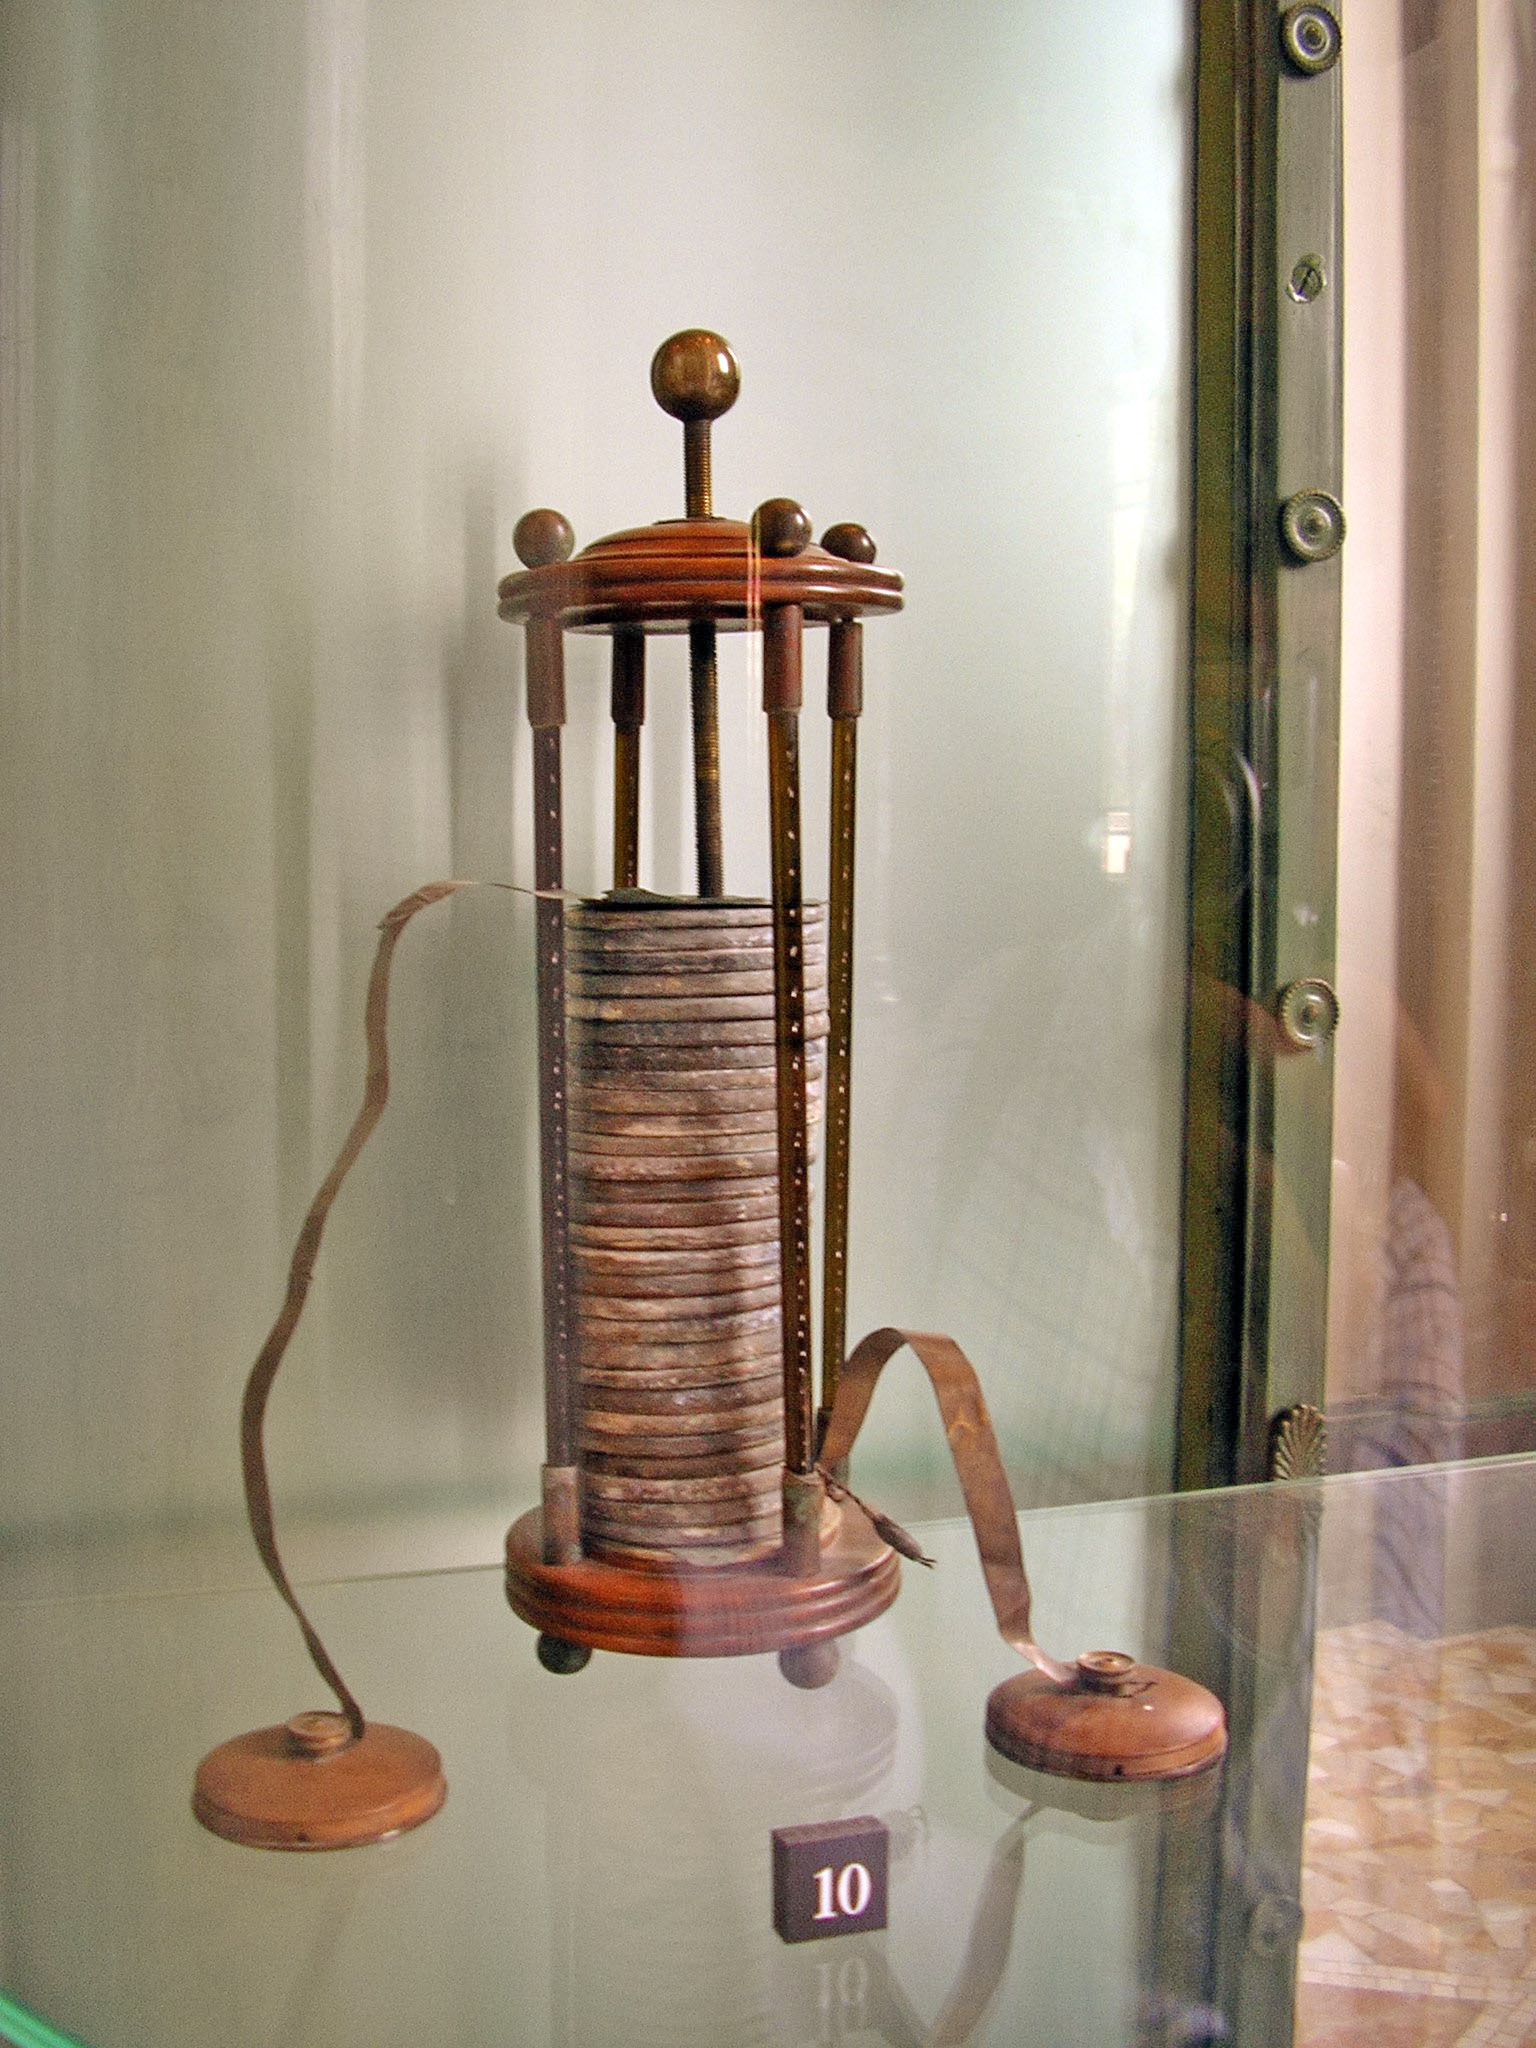
\includegraphics[width=0.24\linewidth]{images/book1/volta-pile.jpg}

{\small Uma pilha de Volta num museu. Foto de GuidoB, CC BY-SA 3.0.}
\end{omfigure}

\section{A tensão de uma pilha}

\begin{definition}[Tensão da pilha]\label{def:g12:cells-and-electrolysis:emf}
A \emph{tensão da pilha}\index{tensao da pilha@tensão da pilha} é a tensão medida entre
os polos de uma pilha que não fornece corrente (circuito aberto), com um
voltímetro; ela é positiva quando o polo positivo do voltímetro está no
\omterm{def:g12:cells-and-electrolysis:anode}{cátodo}.
\end{definition}

\begin{example}[A pilha de Daniell]\label{ex:g12:cells-and-electrolysis:daniell}
% ledger: e0:Cu, e0:Zn, emf:Daniell
Com as duas soluções a \qty{1}{mol/L}, a pilha de Daniell dá
\qty{1.10}{V}. Como prever uma tensão assim a partir de tabelas de
potenciais de eletrodo é mostrado no volume do primeiro ano da
universidade.
\end{example}

\begin{remark}[Por que uma pilha se esgota]\label{rem:g12:cells-and-electrolysis:runs-down}
A reação da pilha, \ce{Zn + Cu^{2+} -> Zn^{2+} + Cu}, tem uma constante
$K$ muito grande. Enquanto a pilha funciona, $Q = [\ce{Zn^{2+}}]/[\ce{Cu^{2+}}]$
aumenta, e a reação continua enquanto $Q < K$. Quando um \omterm{def:g7:chemical-reactions:reactant}{reagente} acaba
(o zinco, ou os \omterm{def:g9:ions:ion}{íons} cobre), a corrente para: a pilha está
``descarregada''.
\end{remark}

\section{Carga e capacidade}

\begin{definition}[Constante de Faraday, capacidade]\label{def:g12:cells-and-electrolysis:capacity}
A \emph{constante de Faraday}\index{constante de Faraday} $F$ é a carga
elétrica de um \omterm{def:g10:the-mole:amount}{mol} de \omterm{def:g9:inside-the-atom:nucleus}{elétrons}, $F = N_A e = \qty{96485}{C/mol}$. A
\emph{capacidade}\index{capacidade} de uma pilha é a maior carga elétrica
que ela pode fornecer, muitas vezes dada em ampères-horas: $\qty{1}{A.h} = \qty{3600}{C}$.
\end{definition}

\begin{proposition}[Carga e quantidade de matéria de elétrons]\label{prop:g12:cells-and-electrolysis:charge}
% ledger: const:F, const:NA, const:e
Uma corrente $I$ que passa durante um tempo $\Delta t$ transporta a
carga $Q = I\,\Delta t$, isto é, uma \omterm{def:g10:the-mole:amount}{quantidade de matéria} de \omterm{def:g9:inside-the-atom:nucleus}{elétrons}
\[
  n(e^-) = \frac{Q}{F} = \frac{I\,\Delta t}{F} .
\]
\end{proposition}

\begin{proof}
Cada \omterm{def:g9:inside-the-atom:nucleus}{elétron} carrega a carga elementar $e$; $n$ \omterm{def:g10:the-mole:amount}{mols} de \omterm{def:g9:inside-the-atom:nucleus}{elétrons}
carregam $n N_A e = n F$.
\end{proof}

\begin{example}[A capacidade de uma pilha de Daniell]\label{ex:g12:cells-and-electrolysis:capacity}
% ledger: aw:Zn, const:F
O eletrodo de zinco contém \qty{6.5}{g} de zinco que pode reagir, isto
é, $6.5/65.4 = \qty{0.099}{mol}$. Cada \omterm{def:g7:atoms-and-molecules:atom}{átomo} de zinco cede dois
\omterm{def:g9:inside-the-atom:nucleus}{elétrons}: $n(e^-) = \qty{0.199}{mol}$, logo $Q = 0.199 \times 96485 = \qty{1.9e4}{C}$,
cerca de $\qty{1.9e4}{}/3600 = \qty{5.3}{A.h}$, se os \omterm{def:g9:ions:ion}{íons} cobre não
acabarem antes.
\end{example}

\section{A eletrólise}

\begin{definition}[Eletrólise, acumulador]\label{def:g12:cells-and-electrolysis:electrolysis}
Uma \emph{eletrólise}\index{eletrolise@eletrólise} é uma \omterm{def:g11:redox:reaction}{reação de oxirredução}
forçada por um gerador elétrico, no sentido oposto ao que ela tomaria
sozinha. Um \emph{acumulador}\index{acumulador} é uma pilha que pode ser
recarregada: durante a carga, o gerador força a sua reação no sentido
inverso, como uma eletrólise.
\end{definition}

\begin{inthelab}[A eletrólise da água]
Dois eletrodos ficam mergulhados em água tornada condutora com um pouco
de sulfato de sódio, cada um sob um tubo de ensaio invertido cheio da
solução. Com um gerador de alguns volts, sobem bolhas dos dois
eletrodos: no \omterm{def:g12:cells-and-electrolysis:anode}{cátodo} (ligado ao polo $-$), gás hidrogênio; no \omterm{def:g12:cells-and-electrolysis:anode}{ânodo}, gás
oxigênio, o primeiro em quantidade duas vezes maior que o segundo. Uma
tala acesa produz um estalo no primeiro gás; uma tala em brasa volta a
se acender no segundo.
\end{inthelab}

\begin{omfigure}
\begin{tikzpicture}[font=\small, scale=1.2]
  % a trough of water, two inverted tubes standing in it
  \fill[omWater] (-1.4,0) rectangle (1.4,1.1);
  \foreach \x/\g in {-0.6/1.2, 0.6/0.6} {
    \fill[omWater] (\x-0.18,0.3) rectangle (\x+0.18,2.9);
    \fill[white] (\x-0.18,{2.9-\g}) rectangle (\x+0.18,2.9);
    \fill[white] (\x,2.9) circle (0.18);
    \draw[om glass] (\x-0.18,0.3) -- (\x-0.18,2.9) arc[start angle=180, end angle=0, radius=0.18] -- (\x+0.18,0.3);
  }
  \draw[om glass] (-1.5,1.25) -- (-1.4,1.15) -- (-1.4,0) -- (1.4,0) -- (1.4,1.15) -- (1.5,1.25);
  \fill[black!55] (-0.65,0) rectangle (-0.55,0.6);
  \fill[black!55] (0.55,0) rectangle (0.65,0.6);
  \node[draw, fill=white, minimum width=1.6cm, minimum height=0.45cm, font=\footnotesize] (g) at (0,-0.75) {gerador};
  \draw[black!70, thick] (-0.6,0) -- (-0.6,0 |- g.north);
  \draw[black!70, thick] (0.6,0) -- (0.6,0 |- g.north);
  \node[font=\footnotesize] at (-0.78,-0.3) {$-$};
  \node[font=\footnotesize] at (0.78,-0.3) {$+$};
  \node[anchor=east, align=right] at (-0.95,2.5) {gás hidrogênio\\ (cátodo)};
  \node[anchor=west, align=left] at (0.95,2.5) {gás oxigênio\\ (ânodo)};
\end{tikzpicture}

{\small A \omterm{def:g12:cells-and-electrolysis:electrolysis}{eletrólise} da água: acima dos eletrodos se junta duas vezes
mais gás hidrogênio que gás oxigênio.}
\end{omfigure}


\begin{example}[A água, dividida]\label{ex:g12:cells-and-electrolysis:water}
No \omterm{def:g12:cells-and-electrolysis:anode}{cátodo}: \ce{2H2O + 2e- -> H2 + 2OH-}; no \omterm{def:g12:cells-and-electrolysis:anode}{ânodo}:
\ce{6H2O -> O2 + 4H3O+ + 4e-}. Para quatro \omterm{def:g9:inside-the-atom:nucleus}{elétrons}, duas \omterm{def:g7:atoms-and-molecules:molecule}{moléculas} de
gás hidrogênio e uma de gás oxigênio, enquanto os \omterm{def:g9:ions:ion}{íons} \ce{H3O+} e
\ce{OH-} formados nos dois eletrodos se recombinam em água: no total,
\ce{2H2O -> 2H2 + O2}, o
inverso da \omterm{def:g4:what-a-fire-needs:burning}{combustão} do hidrogênio, que precisa de energia para
acontecer.
\end{example}

\begin{method}[A massa depositada por uma eletrólise]\label{met:g12:cells-and-electrolysis:mass}
\begin{enumerate}
  \item Escreva a \omterm{def:g11:redox:couple}{semirreação} no eletrodo onde o \omterm{def:g9:periodic-table-first-look:metal}{metal} se forma, por
        exemplo \ce{Cu^{2+} + 2e- -> Cu}.
  \item Calcule a carga $Q = I \Delta t$ e $n(e^-) = Q/F$.
  \item Divida pelo número de \omterm{def:g9:inside-the-atom:nucleus}{elétrons} por \omterm{def:g7:atoms-and-molecules:atom}{átomo}: $n(\ce{Cu}) =
        n(e^-)/2$; depois $m = n \times M$.
\end{enumerate}
\end{method}


\begin{example}[O refino do cobre]\label{ex:g12:cells-and-electrolysis:refining}
% ledger: aw:Cu, const:F
O cobre impuro que sai da fundição é usado como \omterm{def:g12:cells-and-electrolysis:anode}{ânodo} de uma cuba de
\omterm{def:g12:cells-and-electrolysis:electrolysis}{eletrólise} com solução de sulfato de cobre, e uma folha fina de cobre
puro como \omterm{def:g12:cells-and-electrolysis:anode}{cátodo}. No \omterm{def:g12:cells-and-electrolysis:anode}{ânodo}, o cobre \omterm{def:g2:mixing-and-dissolving:dissolve}{se dissolve},
\ce{Cu -> Cu^{2+} + 2e-}; no \omterm{def:g12:cells-and-electrolysis:anode}{cátodo}, cobre puro se deposita,
\ce{Cu^{2+} + 2e- -> Cu}; as impurezas caem no fundo ou ficam em
solução. Uma corrente de \qty{100}{A} durante \qty{24}{h} transporta
$Q = 100 \times 86400 = \qty{8.64e6}{C}$, isto é,
$n(e^-) = \qty{89.5}{mol}$, que deposita $89.5/2 = \qty{44.8}{mol}$ de
cobre: \qty{2.84}{kg}.
\end{example}

\begin{omfigure}
\begin{tikzpicture}[font=\small, scale=1.25]
  \pic[transform shape] at (0,0) {beaker={0.75}{cyan!70!blue!35}};
  \pic[transform shape] (an) at (-0.4,0.2) {electrode={orange!40!brown!80!black}};
  \pic[transform shape] (ca) at (0.4,0.2) {electrode={orange!80!brown}};
  \foreach \p in {(-0.6,0.08),(-0.5,0.12),(-0.3,0.07),(-0.2,0.1)} \fill[black!55] \p circle (0.03);
  \node[draw, fill=white, font=\footnotesize, minimum width=1.6cm] (g) at (0,3.4) {gerador};
  \draw[black!70, thick] (an-top) -- (an-top |- g.south);
  \draw[black!70, thick] (ca-top) -- (ca-top |- g.south);
  \node[font=\footnotesize] at (-0.58,2.95) {$+$};
  \node[font=\footnotesize] at (0.58,2.95) {$-$};
  \draw[omProp, thick, <-] (-0.55,1.2) -- (-1.6,1.6) node[left, align=right, text=black] {ânodo de cobre\\ impuro: se dissolve};
  \draw[omProp, thick, <-] (0.55,1.2) -- (1.6,1.6) node[right, align=left, text=black] {cátodo de cobre\\ puro: cresce};
  \draw[omProp, thick, <-] (-0.35,0.1) -- (-1.6,0.3) node[left, text=black] {impurezas};
\end{tikzpicture}

{\small O refino do cobre por \omterm{def:g12:cells-and-electrolysis:electrolysis}{eletrólise}: o cobre passa do \omterm{def:g12:cells-and-electrolysis:anode}{ânodo} impuro
para o \omterm{def:g12:cells-and-electrolysis:anode}{cátodo} puro através da solução.}
\end{omfigure}

\section{Pilhas, baterias recarregáveis e células a combustível}

Toda pilha ou bateria descartável é uma \omterm{def:g12:cells-and-electrolysis:cell}{pilha eletroquímica}; toda
bateria recarregável, um \omterm{def:g12:cells-and-electrolysis:electrolysis}{acumulador}. A bateria de chumbo-ácido de um
carro funciona com chumbo, óxido de chumbo e ácido sulfúrico; a bateria
de \omterm{def:g9:ions:ion}{íons} de lítio de um celular desloca \omterm{def:g9:ions:ion}{íons} lítio entre dois eletrodos,
um de grafite e outro de um óxido metálico, através de um eletrólito
líquido ou polimérico, enquanto os \omterm{def:g9:inside-the-atom:nucleus}{elétrons} dão a volta pelo circuito
externo. Uma célula a \omterm{def:g4:what-a-fire-needs:fuel}{combustível} é uma pilha cujos \omterm{def:g7:chemical-reactions:reactant}{reagentes} são
alimentados continuamente: uma célula a \omterm{def:g4:what-a-fire-needs:fuel}{combustível} de hidrogênio
realiza a reação \ce{2H2 + O2 -> 2H2O}, o inverso da \omterm{def:g12:cells-and-electrolysis:electrolysis}{eletrólise} da água,
e fornece eletricidade e água. O gás hidrogênio produzido por \omterm{def:g12:cells-and-electrolysis:electrolysis}{eletrólise}
com eletricidade do vento ou do Sol, e depois usado em células a
\omterm{def:g4:what-a-fire-needs:fuel}{combustível}, é uma maneira de armazenar essa eletricidade.

\begin{omfigure}
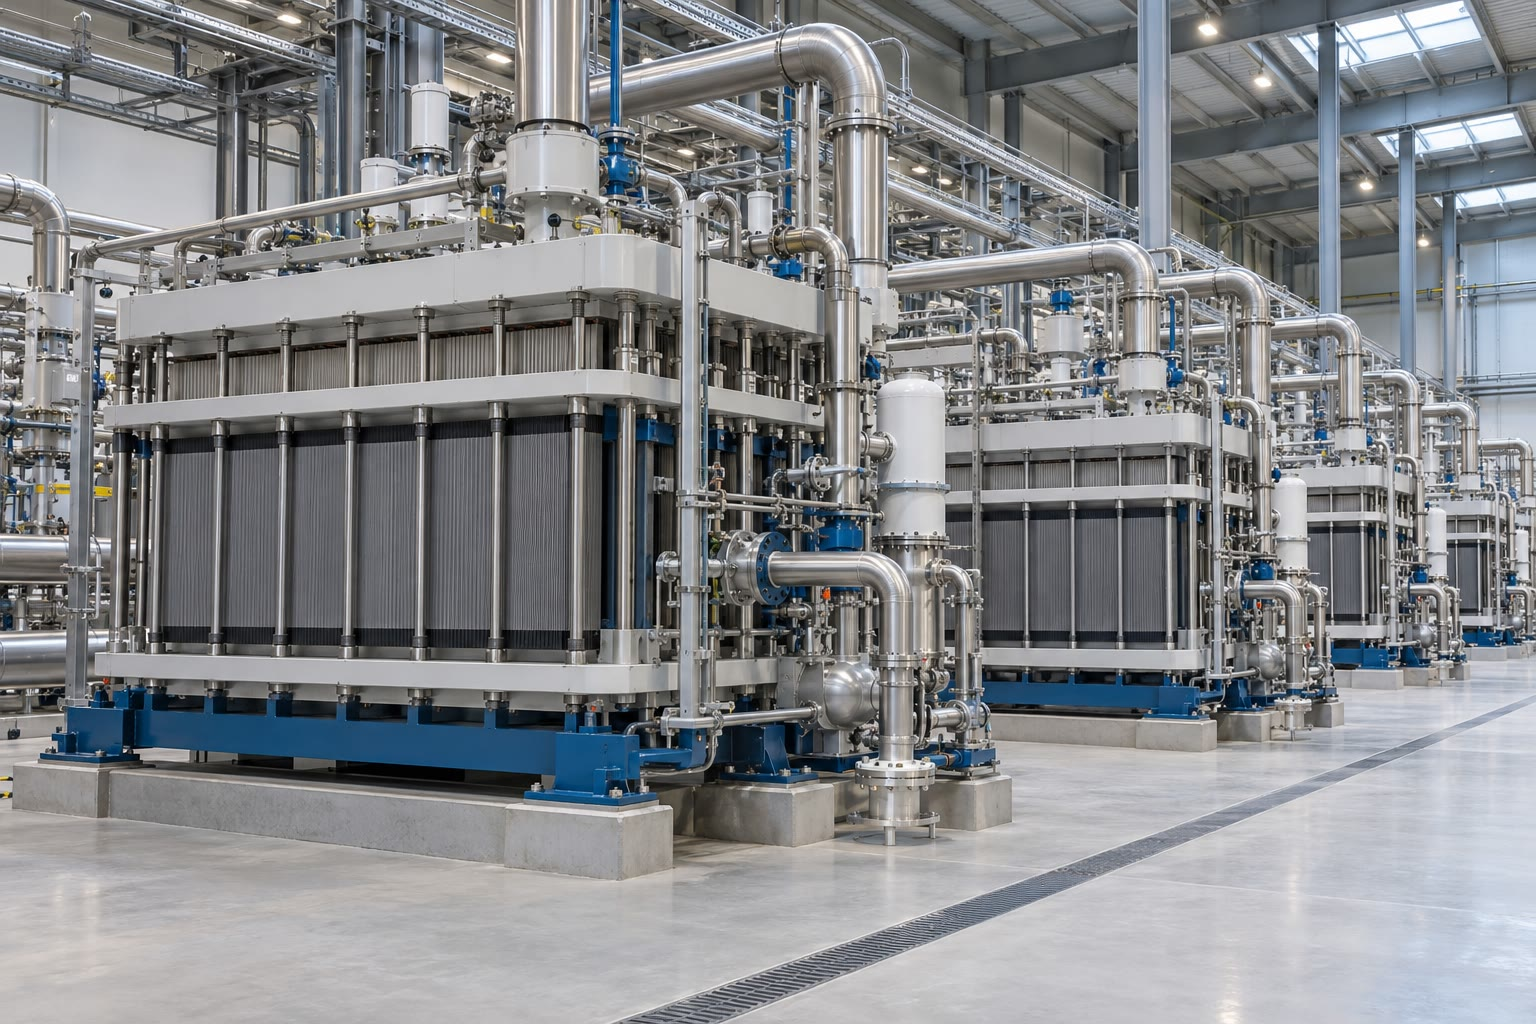
\includegraphics[width=0.48\linewidth]{images/book1/ai/g12-electrolyser-hall.jpg}

{\small Um galpão de eletrolisadores: a água é dividida em gás
hidrogênio e gás oxigênio.}
\end{omfigure}

\section{Exercícios}

\begin{exercise}[$\star$]\label{exo:g12:cells-and-electrolysis:1}
Na pilha de Daniell, que eletrodo é o \omterm{def:g12:cells-and-electrolysis:anode}{ânodo}? E o \omterm{def:g12:cells-and-electrolysis:anode}{cátodo}? Escreva a
\omterm{def:g11:redox:couple}{semirreação} em cada um.
\end{exercise}

\begin{exercise}[$\star$]\label{exo:g12:cells-and-electrolysis:2}
Uma corrente de \qty{0.20}{A} passa durante \qty{30}{min}. Calcule a
carga transportada e a \omterm{def:g10:the-mole:amount}{quantidade de matéria} de \omterm{def:g9:inside-the-atom:nucleus}{elétrons}.
\end{exercise}

\begin{exercise}[$\star$]\label{exo:g12:cells-and-electrolysis:3}
Qual é o papel da \omterm{def:g12:cells-and-electrolysis:cell}{ponte salina}? O que acontece se ela for retirada?
\end{exercise}

\begin{exercise}[$\star$]\label{exo:g12:cells-and-electrolysis:4}
Converta uma \omterm{def:g12:cells-and-electrolysis:capacity}{capacidade} de \qty{2.5}{A.h} em coulombs.
\end{exercise}

\begin{exercise}[$\star$]\label{exo:g12:cells-and-electrolysis:5}
Numa \omterm{def:g12:cells-and-electrolysis:electrolysis}{eletrólise}, a reação é espontânea? O que fornece a energia?
\end{exercise}

\begin{exercise}[$\star\star$]\label{exo:g12:cells-and-electrolysis:6}
Uma pilha é feita de um eletrodo de prata em nitrato de prata e de um
eletrodo de cobre em sulfato de cobre. O voltímetro mostra que os
\omterm{def:g9:inside-the-atom:nucleus}{elétrons} saem pelo cobre. Escreva as \omterm{def:g11:redox:couple}{semirreações}, dê o nome do \omterm{def:g12:cells-and-electrolysis:anode}{ânodo} e
do \omterm{def:g12:cells-and-electrolysis:anode}{cátodo}, e dê a reação global.
\end{exercise}

\begin{exercise}[$\star\star$]\label{exo:g12:cells-and-electrolysis:7}
Uma bateria de relógio fornece \qty{10}{\micro A} continuamente durante
três anos. Qual é a sua \omterm{def:g12:cells-and-electrolysis:capacity}{capacidade} em \si{mA.h}?
\end{exercise}

\begin{exercise}[$\star\star$]\label{exo:g12:cells-and-electrolysis:8}
Uma colher é prateada com uma corrente de \qty{0.50}{A} durante
\qty{40}{min}, \ce{Ag+ + e- -> Ag}. Que massa de prata é depositada?
\end{exercise}

\begin{exercise}[$\star\star$]\label{exo:g12:cells-and-electrolysis:9}
Na figura da pilha de Daniell, dê o sentido da corrente no fio e o
sentido em que se deslocam os \omterm{def:g9:ions:ion}{íons} \ce{K+} e \ce{NO3-} da ponte.
\end{exercise}

\begin{exercise}[$\star\star$]\label{exo:g12:cells-and-electrolysis:10}
Compare uma pilha e uma \omterm{def:g12:cells-and-electrolysis:electrolysis}{eletrólise}: o sinal do \omterm{def:g12:cells-and-electrolysis:anode}{ânodo}, o sentido da
reação, a conversão de energia.
\end{exercise}

\begin{exercise}[$\star\star$]\label{exo:g12:cells-and-electrolysis:11}
Na \omterm{def:g12:cells-and-electrolysis:electrolysis}{eletrólise} da água, recolhem-se \qty{24}{mL} de gás hidrogênio. Que
volume de gás oxigênio é recolhido ao mesmo tempo? Por quê?
\end{exercise}

\begin{exercise}[$\star\star\star$]\label{exo:g12:cells-and-electrolysis:12}
Uma pilha de Daniell contém \qty{5.0}{g} de zinco e \qty{100}{mL} de
sulfato de cobre a \qty{0.50}{mol/L}. Que \omterm{def:g7:chemical-reactions:reactant}{reagente} acaba primeiro? Qual
é a \omterm{def:g12:cells-and-electrolysis:capacity}{capacidade} da pilha? Durante quanto tempo ela pode fornecer
\qty{50}{mA}?
\end{exercise}

\begin{exercise}[$\star\star\star$]\label{exo:g12:cells-and-electrolysis:13}
Uma pilha de \qty{1.5}{V} fornece \qty{2.0}{A.h}. Calcule a energia que
ela armazena ($E = Q U$), em joules e em watts-hora.
\end{exercise}

\begin{exercise}[$\star\star\star$]\label{exo:g12:cells-and-electrolysis:14}
A água é eletrolisada com \qty{2.0}{A} durante \qty{1.0}{h}. Calcule as
\omterm{def:g10:the-mole:amount}{quantidades de matéria}, e depois os volumes a \qty{20}{\celsius} ($V_m = \qty{24.1}{L/mol}$),
de gás hidrogênio e de gás oxigênio produzidos.
\end{exercise}

\begin{exercise}[$\star\star\star$]\label{exo:g12:cells-and-electrolysis:15}
No refino do cobre, o \omterm{def:g12:cells-and-electrolysis:anode}{ânodo} perde \qty{3.00}{kg} de material enquanto o
\omterm{def:g12:cells-and-electrolysis:anode}{cátodo} ganha \qty{2.84}{kg} de cobre. Qual é a porcentagem de cobre no
\omterm{def:g12:cells-and-electrolysis:anode}{ânodo} impuro, supondo que só o cobre se oxida no \omterm{def:g12:cells-and-electrolysis:anode}{ânodo} e que as
impurezas simplesmente se soltam?
\end{exercise}

\section{Problema: a bateria do celular}

\begin{problem}[{Problema de fim de semana --- que massa de lítio vai e vem
entre os eletrodos de uma bateria de celular de \qty{4000}{mA.h}?}]
\label{pb:g12:cells-and-electrolysis:1}
% ledger: const:F, const:NA, aw:Li, dch:CH4, aw:C, aw:H
Uma bateria de celular traz a indicação ``\qty{3.7}{V}, \qty{4000}{mA.h}''.
Numa imagem simplificada, durante a descarga, cada \omterm{def:g7:atoms-and-molecules:atom}{átomo} de lítio
armazenado no eletrodo de grafite cede um \omterm{def:g9:inside-the-atom:nucleus}{elétron} e sai como \omterm{def:g9:ions:ion}{íon} lítio,
\ce{Li -> Li+ + e-}; o \omterm{def:g9:ions:ion}{íon} atravessa o eletrólito e é captado pelo
eletrodo de óxido metálico, que ganha um \omterm{def:g9:inside-the-atom:nucleus}{elétron} ao mesmo tempo.

\medskip
\noindent\textbf{Parte I --- A pilha.}
\begin{enumerate}
  \item Durante a descarga, o eletrodo de grafite é o \omterm{def:g12:cells-and-electrolysis:anode}{ânodo} ou o
        \omterm{def:g12:cells-and-electrolysis:anode}{cátodo}? Por quê?
  \item Qual é o polo negativo?
  \item Em que sentido os \omterm{def:g9:inside-the-atom:nucleus}{elétrons} percorrem o celular? E os \omterm{def:g9:ions:ion}{íons} lítio
        dentro da bateria?
  \item Por que essa pilha é um \omterm{def:g12:cells-and-electrolysis:electrolysis}{acumulador}?
\end{enumerate}

\medskip
\noindent\textbf{Parte II --- A carga.}
\begin{enumerate}[resume]
  \item Converta \qty{4000}{mA.h} em ampères-horas, e depois em coulombs.
  \item Calcule a \omterm{def:g10:the-mole:amount}{quantidade de matéria} de \omterm{def:g9:inside-the-atom:nucleus}{elétrons} que essa carga
        representa.
  \item Quantos \omterm{def:g9:inside-the-atom:nucleus}{elétrons} são isso?
  \item O celular consome em média \qty{0.25}{A}. Quanto tempo dura uma
        bateria carregada?
  \item A tela mostra 20 \%. Que carga, em coulombs, resta?
\end{enumerate}

\medskip
\noindent\textbf{Parte III --- A energia.}
\begin{enumerate}[resume]
  \item Calcule a energia armazenada, $E = Q U$, em joules.
  \item Converta-a em watts-hora.
  \item Compare com a energia liberada pela \omterm{def:g4:what-a-fire-needs:burning}{queima} de \qty{1}{g} de
        metano (\qty{55.7}{kJ}).
  \item Quantas cargas completas dá \qty{1}{kW.h} de eletricidade, se
        nenhuma energia fosse perdida?
\end{enumerate}

\medskip
\noindent\textbf{Parte IV --- A recarga.}
\begin{enumerate}[resume]
  \item Durante a carga, que reação acontece no eletrodo de grafite? É
        uma \omterm{def:g11:redox:oxidation}{oxidação} ou uma \omterm{def:g11:redox:oxidation}{redução}?
  \item Por que a recarga é uma \omterm{def:g12:cells-and-electrolysis:electrolysis}{eletrólise}?
  \item O carregador fornece \qty{2.0}{A}. Quanto tempo leva, no mínimo,
        uma recarga completa?
  \item Que \omterm{def:g10:the-mole:amount}{quantidade de matéria} de \omterm{def:g9:ions:ion}{íons} lítio atravessa o eletrólito
        durante uma carga completa?
  \item Calcule a sua massa.
  \item Dê a resposta final: que massa de lítio vai e vem entre os
        eletrodos numa carga completa?
\end{enumerate}
\end{problem}
